%%%%%%%%%%%%%%%%%%%%%%%%%%%%%%%%%%%%%%%%%%%%%%%%%%%%%%%%%%%%%%%%
%%                          CHAPTER 2                         %%
%%%%%%%%%%%%%%%%%%%%%%%%%%%%%%%%%%%%%%%%%%%%%%%%%%%%%%%%%%%%%%%%
\chapter{Statistical properties of synchronisers}
Brief explanation of the role of synchronisers in learning for proliferation (that initial throughput value estimation is needed as well as initial channel sizes)

What is a statistical model in general? (See wiki page) How are they used?

The practical side of statistical model:
  \begin{itemize}
  \item The model of the relatioships between various object parameters
  \end{itemize}
%Практический смысл статистической модели:
%1) Характеристики $T'_{i}, \; j'_{i}$ являются начальными значениями для алгоритма пролиферации
%2) Начальные размеры каналов


\section{Statistical model}
%Explaining channels lengths
Let $m$ be the number of input channels of a synchroniser, $n$ be the total number of the synchroniser channels. Then, the number of output channels of the synchroniser is $n-m$. All channels $c_{i}, \; i = 1,n$ are finite FIFO-queues, having lengths $L_i, \; i = 1,n$ as pictured in Fig. \ref{fig:stat_mod}.

% Inkscape figure
  \begin{figure}[h] %here!
  %\centering
  \def\svgwidth{14cm} % используем для изменения размера, если надо
  \includesvg{figs/stat_mod}
  \caption{A statistical model of a synchroniser.}
  \label{fig:stat_mod}
  \end{figure}

%Explaining basic structure of channel and input channel producer properties
Every input channel $c_{i}, \; i = 1,m$ is connected to a producer $C_{i}$, sending to this channel $T_{i}$ messages within a predefined unit of time on average (i.e. with a frequency $T_{i} \; u.o.t^{-1}$) with an independent jitter (standard deviation is meant) $j_{i}$ to this value. $T_{i}$ may as well be interpreted as a throughtput of the producer $C_{i}$. $T_{i}$ and $j_{i}, \; i=1,m$ assume that the channel $c_{i}$ has infinite length.

%From statistics point of view - probably should move this part
This may be understood in a different way: the interarrival time $t_{i}, \; i=1,n$ of messages in a channel $c_{i}$ is distributed according to a two-parameter law (CDF) $F_{i} \: (t < t_{i}) = F_{i} \: (p_{i}, t_{i}, t_{i})$. The interarrival's time expected value is $M[t_{i}] = \frac{1}{T_{i}}$ and its variance is $D[t_{i}] = g \: (j_{i})$ (TODO: find $g(j)$). If a length of a channel where messages are placed by a producer, is finite, then the interarrival time mean should increase.

%Explaining synchroniser consuming characteristics
When messages are placed in a queue in front of a synchroniser, they wait there until it consumes them. In some states synchroniser may block input channels (not accept messages from them). Let $T'_{i}, \; i=1,m$ be the number of messages accepted by a synchroniser in a u.o.t. on average and $j'_{i}$ be a standard deviation of $T'_{i}$.

%Synchroniser producing characteristics
A synchroniser is a producer for its output queues $c_{i}, \; i=m+1,n$. Let $T'_{i}, \; i=m+1,n$ be be the number of messages produced by a synchroniser in the output channel $c_{i}$ in a u.o.t on average, and $j'_{i}$ again be a standard deviation of $T'_{i}$.

%Ouptut channels consumers
Synchroniser's output channels are connected to processes that consume messages from these channels. Let $T_{i}, \; i=m+1,n$ be the number of messages consumed by a consumer process $C_{i}$ in u.o.t on average, and $j'_{i}$ be a standard deviation of $T_{i}$.

%problem statement
\textbf{Problem statement} Find relations between $T_{i}, \; j_{i}, \; T'_{i}$, $j'_{i}$ and $L_{i}, \; i=1,n$.


\textbf{Some obvious properties of the model}
Let $l_{i}, \; i = 1,n$ be the actual number of messages stored in any moment of time in channels $L_{i}$. Then the following is true:
  \begin{itemize}
  \item If anytime $l_{i} < L_{i}$, then $T'_{i} = T_{i}$, $i = 1,m$;
  \item If sometime $l_{i} = L_{i}$, then $T'_{i} < T_{i}$, $i = 1,m$;
  \item If $l_{i} > 0$, then $T'_{i} = T_{i}$, $i = m+1,n$;
  \item If $l_{i} = 0$, then $T'_{i} < T_{i}$, $i = m+1,n$.
  \end{itemize}

\section{Relevant work}
TODO

\section{The plan of study}
%TODO: These all need better explanation w.r.t (Some obvious properties of the model)
%Influence of finite input channel lengths on producers
$T_{i}$ and $j_{i}, \; i=1,m$ are the characteristics of producers in assumption that the channels $c_{i}, \; i=1,m$ they are connected to, are infinite. A finite channel length affects these values. If a channel is full, messages can't be placed in it anymore, so $T_{i}$ decreases. (TODO: what happens to $j_{i}$, does it decrease as well?)

%Synchroniser input characteristics
The affected values $T_{i}, \; j_{i}, \; i=1,m$ change $T'_{i}, \; j'_{i}$. Also $T'_{i}$ and $j'_{i}$ are affected by the transition diagram of a synchroniser causing input channel blockings.

%Influence of finite output channel lengths on synchroniser
If output channels of a synchroniser have finite lengths, it affects the output characteristics of a synchroniser $T'_{i}$ and $j'_{i}, \; i=m+1,n$ as finite input channels lengths affect producers.

%Influence on synchroniser consumers
The characteristics of synchroniser consumers are not affected directily by finite channels lengths. They are directly affected by $T'_{i}$ and $j'_{i}, \; i=m+1,n$.


%The plan of study
%What kind of synchronisers is studied
In this project we study only synchronisers whose transition diagrams have deterministic transitions, i.e a transition diagram doesn't depend on message content. If more that one transition possible at the same time, than all choices are made with the same frequency.

%Describe the idea for a study. We have 3 problems with a synchroniser: input channels are finite, transition diagram is random (fixed by the language), output channels are finite. Decribe the order in which these problems are studied (the strategy).

We break down the problem into parts:
  \begin{enumerate}
  \item Study the part of a system that doesn't depend on the output channels
    \begin{itemize}
    \item Find $T'_{i}$ and $j'_{i}, \; i=1,m$ depending on $T_{i}, \; j_{i}, \; i=1,m$ and finite channel lengths $L_{i}, \; i=1,m$;
    \item Investigate how $T_{i}, \; j_{i}, \; i=1,m$ are affected by $L_{i}, \; i=1,m$;
  \end{itemize}

  \item Study the part of a system that depends on the output channels
    \begin{itemize}
    \item Find "ideal" $T'_{i}$ and $j'_{i}, \; i=m+1,n$ with assumption that output channels have infinite lengths;
    \item Study an impact of finite output channels on $T'_{i}$ and $j'_{i}, \; i=m+1,n$;
    \item Investigate how $T_{i}$ and $j_{i}, \; i=m+1,n$ of consumers are affected.
    \end{itemize}
  \end{enumerate}


\section{Modeling a system}

  \subsection{Modeling channels}
Channels act as FIFO-queues. Message arrivals in a channel are independent events with interarrival time $\Delta t$ distributed according to the gamma distribution: $\Delta t \sim Gamma (k, \theta, t)$. Gamma distribution is chosen because of two reasons:
    \begin{itemize}
    \item it is a well-studied distribution that generates positive values, i.e. its domain of definition is $t \in [0;\infty]$, and interarrival times must be positive,
    \item it is closed to the convolution operation if the parameter $\theta$ is fixed: $Gamma_(k_{1}, \theta) * Gamma (k_{2}, \theta) = Gamma (k_{1} + k_{2}, \theta)$; this property helps to significantly simplify heavy computations involving convolutions.
    \end{itemize}

According to the central limit theorem, any distribution could be chosen -- it should not change results significantly. (Explain why?)

TODO Put a graph somewhere with the number of messages in a channel over time (the channel is finite and connected to a synchroniser) Probably appendix with the Brownian motion

  \subsection{Modeling artificial load}
Describe the modeling of a synchroniser with a general case transition diagram (data structures, algorithms, tools, etc)
    \begin{itemize}
    \item For the unlimited queue
    \item For the limited queue
    \end{itemize}

  \subsection{Limitations of the model}
Describe the limitations of this model (only considers choosing a transition by choice frequency if more than one channel are ready)


\section{Application of Markov chains to synchronisers}
In this section we explain how to find $T'_{i}$ and $j'_{i}, \; i=1,n$ using Markov chains.
  \subsection{Introduction to Markov chains}
A short introduction to discrete and continuous Markov networks.

\textbf{Discrete Markov chains}
Discrete: the states and the transition probability matrix $P$. The transition probabilities do not depend on how the state was reached. The matrix $P$ has the following properties: the sum of all elements in each raw is 1, and $lim_{n - \infty} P = P_{steady}$. The elements in each column of the matrix $P_{steady}$ have the same value and the sum of elements in (each) raw is 1. These probabilities are called steady state probabilities.

\textbf{Continous Markov chains}
TODO

  \subsection{States of a chain}
States of channels
Describe what are the states of the chain ($A_{i} B_{j} L_{k}$). How the number of states depends on the length of the channels. Why number of states is unlimited (because of $L_{k}$).

Example: zip2
  \subsection{Simplification}
-discrete time
-events in channels

Describe the continous case first. Show that why the discretisation is reasonable.
Describe the discrete case. How $L_{k}$ is cut (by choosing possible events $(n,a,b,ab,...)$)

How we chose the set of possible events. We want the most minimal set possible that shows the dependence of steady-state probabilities on the distribution parametes.

%TODO: Come up with a good name for it
  \subsection{How to find $T'$ and $j'$}
TODO
dT = $\frac{sum of steady-state probabilities where messages are lost)}{t_{t}}$

\section{Example: application of the Markov chain to the zip2 synchroniser}
  \subsection{Modeling the throughput}
$T = T \: (\sigma, l)$, where $\sigma = \sigma_{a} = \sigma_{b}$ - variance in both channels, $l = l_{a} = l_{b}$ - length of both channels. See \ref{fig:t_s}
    \begin{figure}[here]
    \centering
    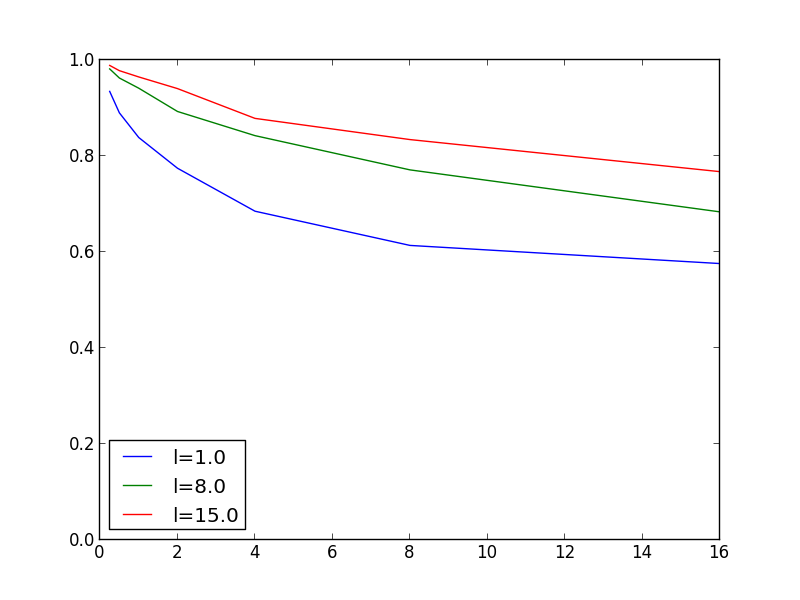
\includegraphics[scale=0.4]{figs/thr_(disp,l).png}
    \caption{$T = T \: (\sigma, l)$.}
    \label{fig:t_s}
    \end{figure}

Explain the shape of the graph when $\mu \sim \sigma$ or $\mu >> \sigma$.
Plot a graph for $0 < \sigma < \frac{\mu}{2}$.

  \subsection{Analytical results}
-States of the chain
Why we do not consider lost messages separately for each channels in the case of zip2. 

-events in channel (the minimal set for the zip2 synchroniser)
First, we try the most minimalistic set $(n,a,b)$. Let $F_{a}(t) = Gamma(k, \theta, t)$ the distribution of interarrival times in the channels. Then the probability of one message $a$ coming to the channel $A$ in time $t_{t}$ $P_{a} = F_{a}(t_{t}) = Gamma(t_{t})$. The same is for a message $b$ coming to the channel $B$ in time $t_{t}$: $P_{b} = F_{b}(t_{t}) = Gamma(t_{t})$. Note that the discretion time $t_{t}$ must be chosen so that the ptobability os an event $ab$ in time $t_{t}$ is almost zero: $P_{ab}(t_{t}) = convolution! Gamma(t_{t})^2$. The probability to see the event $a$ arrived in $A$, channel $B$ is empty $P_{a} = Gamma(t_{t})(1-Gamma(t_{t})) = Gamma(t_{t}) - Gamma(t_{t})^2 \sim Gamma(t_{t})$. The probability to see the event $n$ (nothing arrived) in the channels over time $t_{t}$ $P_{n} = (1-p)^2 = 1 - 2 Gamma(t_{t}) + Gamma(t_{t})^2 \sim 1 - 2 Gamma(t_{t})$. The total probability of all possible events in the system $P_{n} + P_{a} + P_{b} = 1 - 2 Gamma(t_{t}) + Gamma(t_{t}) + Gamma(t_{t}) = 1$ as it should be. Then we fill the Markov transition probabilities matrix $P$ for the system's states and solve the matrix equation $xP = x$. Then we find that steady-state probabilities do not depend on the parameters of the distribution in the channels which means that we should consider more events.

Then we take the set of events $(n,a,b,ab)$, for which $P_{a} = P_{b} = Gamma(t_{t})(1 - Gamma(t_{t}))$, $P_{ab} = Gamma(t_{t})^2$ and $P_{n} = (1 - Gamma(t_{t}))^2$. For this set we see the dependence of the steady-state probabilities on $Gamma(t_{t})$.

-time $t_t$
If we expect just one message to come to a channel, then we may take the expected mean of the distribution as the discretion time $t_{t} \sim m(Gamma(k,\theta)) = k \theta$.


Build $P_{steady}$, solve $x P_{steady} = x$, dT = $\frac{\sum{x_l}}{t_t}$, $T' = T - dT$.

Expand $T'$ for $\sigma << \mu$. Plot two graphs on the same picture.

\section{Good-enough channel length?}
$l \sim \frac{Dk}{\langle k \rangle}$, where $Dk = \sum_{k} (k - \langle k \rangle)^{2} a_{k}$, $\langle k \rangle = \sum_{k} k a_{k}$.
